\chapter{Climate Risk}

Pastor \textit{et al.} extends their theoretical framework
by allowing climate to enter investors' utility. 
Expected returns then depend not only on market betas 
but also on climate betas, which measure firms' exposure 
to climate shocks. According to the authors, 
evidence suggests that brown assets have 
higher climate betas than green assets.
This difference pushes up brown assets' expected returns in 
PST model. The idea is that investors dislike unexpected 
deteriorations in the climate. If the climate 
worsens unexpectedly, brown assets lose value relative 
to green assets. Because brown firms lose values in 
state of the world investors dislike, they are riskier, 
so they must offer higher expected returns to compensate
investors for bearing this risk.

\begin{figure}[htbp]
    \centering
    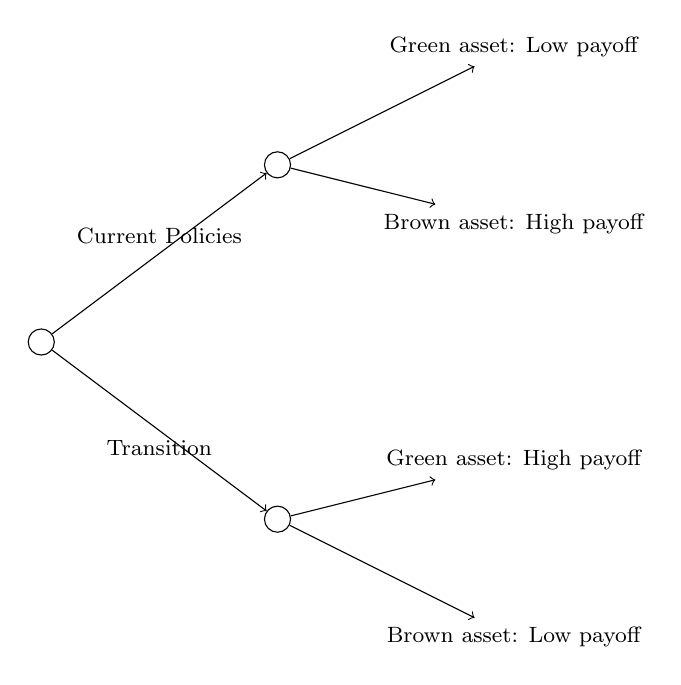
\begin{tikzpicture}[scale=1.5, every node/.style={font=\footnotesize}]

    % Nodes
    \node (start) at (0,0) [draw, circle] {};
    \node (current) at (2,1.5) [draw, circle] {};
    \node (transition) at (2,-1.5) [draw, circle] {};
    \node (current_green) at (4,2.5) {Green asset: Low payoff};
    \node (current_brown) at (4,1) {Brown asset: High payoff};
    \node (transition_green) at (4,-1) {Green asset: High payoff};
    \node (transition_brown) at (4,-2.5) {Brown asset: Low payoff};

    % Edges
    \draw[->] (start) -- (current) node[midway, above] {Current Policies};
    \draw[->] (start) -- (transition) node[midway, below] {Transition};
    \draw[->] (current) -- (current_green);
    \draw[->] (current) -- (current_brown);
    \draw[->] (transition) -- (transition_green);
    \draw[->] (transition) -- (transition_brown);
    
    % Labels

\end{tikzpicture}
    \caption{Climate States of the World}
    \label{fig:climate_risk}
\end{figure}


\section{Brown / Green Assets}

\section{Climate Risk and Utility}



\section{Climate Betas and Expected Returns}